\section{Direct lattice}

\vspace*{0.5cm}
\begin{center}
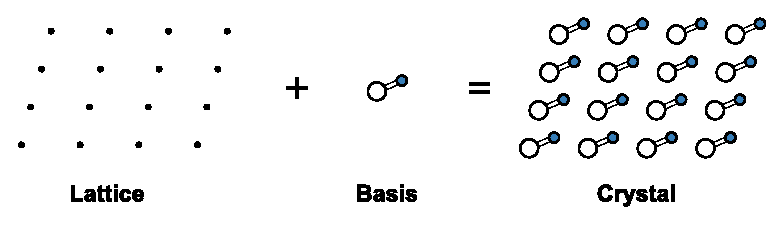
\includegraphics[width=0.75\textwidth]{crystal_structure/figures/crystal.eps}
\end{center}

\noindent
The mathematical description of the crystal consists of two parts: the \emph{lattice} which is a periodic grid of points extending over space and the \emph{basis} which in this context is the set of ions repeating at every lattice point.

The lattice can be described by the set of so called \emph{lattice vectors} $\lbrace\mathbf{R}\rbrace$ given by
\begin{equation}
\mathbf{R} \equiv \mathbf{R}_{n_1 n_2 n_3}  = n_1 \mathbf{a}_1 + n_2 \mathbf{a}_2 + n_3 \mathbf{a}_3,
\end{equation}
where $n_i \in \mathds{Z}$ and $\mathbf{a}_i$ are linearly independent vectors in the real space called the \emph{primitive vectors}. The primitive vectors have the dimensions of length owing to which the lattice spanned by them is referred to as the \emph{direct lattice}. It should be noted the choice of the primitive vectors is not unique; any non-collinear set of the lattice vectors can be used.

The lattice can be infinite or finite depending on the allowed values of $n_i$. Quite often it is convenient to deal with infinite lattice which extends over all spatial dimensions. In such case the lattice is known as the \emph{Bravais lattice}. 

An important concept of \emph{unit cell} builds upon the lattice. A unit cell is a volume of space that can fill the entire space without overlaps or leaving gaps behind when translated by a suitable set of Bravais lattice vectors. A \emph{primitive unit cell} is a special set of unit cells which enclose precisely one lattice point. Therefore, if the number density of lattice points is $n$, the primitive unit cell volume $v$ is 
\begin{equation}
v = \frac{1}{n}
\end{equation}
regardless the shape of the cell. Sometimes it is, however, easier to work with a \emph{conventional unit cell} instead. For example, a primitive unit cells of a BCC (body-centered cubic) lattice can be difficult to work with since their angles are not orthogonal. The usual choice is to use a cubical cell containing two lattice points instead. Note that whereas primitive unit cells can be translated by all the lattice vectors without any overlaps, the same is not true for the conventional ones. 

There is, however, a common used way to choose a primitive unit cell that has the full symmetry of the lattice. Consider a single lattice point and take all the points in its vicinity that are nearer to it than any other point in the lattice. The volume covered by those points leads to a unique primitive unit cell which is known as the \emph{Wigner-Seitz cell}. The concept is worth remembering as it has an important role in the subsequent discussion.

\vspace*{0.5cm}
\begin{figure}[h!]
\centering

\includegraphics[width=0.4\textwidth]{crystal_structure/figures/wigner-seitz.eps}
\caption{Wigner-Seitz cell of an oblique 2D-lattice. The blue area covers the points closest to the lattice point in the center.}
\end{figure}


\bibliographystyle{plain}
%\bibliography{magnetism/refs}
 